\section{Gruppen}

\begin{definition}
    Sei $\mathfrak{G} = (G, \cdot, e, {}^{-1})$ eine Gruppe.
    \begin{itemize}
        \item Wir nennen $|G|$ die \emph{Ordnung} der Gruppe.\index{Gruppe!Ordnung}
        \item Sei $g \in G$, so erzeugt dieses Element eine Untergruppe
        $$ \langle \{ g \} \rangle = \{ g^n \mid n \in \mathbb{Z} \}. $$
        Wir nennen $|\langle\{g\}\rangle|$ die \emph{Ordnung} von $g$ und schreiben auch $\ord(g)$. Ist $\ord(g)$ endlich, so heißt $g$ \emph{Torsionselement}.\index{Gruppe!Torsionselement}
        \item $\mathfrak{G}$ heißt \emph{zyklisch}, falls es ein $g \in G$ mit $G = \langle\{g\}\rangle$ gibt.\index{Gruppe!zyklisch}
    \end{itemize}
\end{definition}

\begin{remark}
    Im Folgenden werden wir Gruppen durch ihre Trägermengen identifizieren. Für die Gruppe $\mathfrak{G} = (G, \cdot, e, {}^{-1})$ wird oft nur $G$ geschrieben.
\end{remark}

\begin{example} {\ }
    \begin{enumerate}
        \item Betrachte $\mathbb{Z} \times \mathbb{Z}_m$, so ist $\ord(1,0) = \infty$ und $\ord(0,1) = m$.
        \item Betrachte $\mathbb{Z}_6$, so ist $\ord(1) = 6$, $\ord(2) = 3$ und $\ord(3) = 2$.
    \end{enumerate}
\end{example}

\begin{example} {\ }
    \begin{enumerate}
        \item Die Gruppen $(\mathbb{Z}, +, 0, -) = \langle\{1\}\rangle, (\mathbb{Z}_m, +, 0, -) = \langle\{1\}\rangle$ sind zyklisch.
        \item Die Gruppe $(\Gl_2(\mathbb{Q}), \cdot, E_2, {}^{-1})$ ist \emph{nicht} zyklisch, da -- wie wir noch sehen werden -- zyklische Gruppen abelsch sind.
    \end{enumerate}
\end{example}

\notedate{30.03.2023}

\begin{definition}
    Seien $G$ eine Gruppe, $U \le G$ eine Untergruppe und $g \in G$. Wir definieren 
    \begin{itemize}[topsep=0cm, label={--}]
        \item die \emph{Linksnebenklasse von $g$ nach $U$}\index{Linksnebenklasse} $gU := \{gu \mid u \in U\}$ und
        \item die \emph{Rechtsnebenklasse von $g$ nach $U$}\index{Rechtsnebenklasse} $Ug := \{ug \mid u \in U\}$.
    \end{itemize}
\end{definition}

\begin{lemma}\label{lemma:euqivrel_linksnebenklassen}
    Seien $G$ eine Gruppe, $U \le G$ eine Untergruppe und $g, g', x, y \in G$. Dann gilt:
    \begin{enumerate}
        \item Die Menge $\{gU \mid g \in G\}$ aller Linksnebenklassen von $g$ nach $U$ bildet eine Partition von $G$.
        \item Es gilt $gU = g'U$ genau dann, wenn $g^{-1}g' \in U$.
        \item Die Partition induziert eine Äquivalenzrelation $\sim$ auf $G$, wobei $x \sim y \Leftrightarrow \exists \tilde{g} \in G: x,y \in \tilde{g}U$.
        \item Es gilt für diese Äquivalenzrelation $x \sim y \Leftrightarrow x^{-1}y \in U$.\label{item:lemma:euqivrel_linksnebenklassen_4}
        \item Es ist $U = [e]_{\sim}$.
    \end{enumerate}
    
\end{lemma}
\begin{proof}{\ }
    \begin{enumerate}
        \item Es gilt $G = \bigcup_{g \in G} gU$, denn für $h \in G$ ist $h \in hU$, weil $e \in U$ und $h = h \cdot e$ ist. 
        
        Es bleibt noch zu zeigen, dass die Nebenklassen disjunkt sind. Dafür zeigen wir, dass nicht disjunkte Linksnebenklassen gleich sind. Seien also $g, g' \in G$ beliebig mit $gU \cap g'U \not= \emptyset$. Es existieren dann $u, u' \in U$, sodass $g u = g' u'$. Sei $a = g  u_a \in gU$ beliebig. Es ist dann $$ a = g u_a = g u u^{-1} u_a = g' \underbrace{u' u^{-1} u_a}_{\in U} \in g'U, $$
        also $gU \subseteq g'U$. Analog erhält man die andere Mengeninklusion, womit $gU = g'U$ gilt.
        \item Es ist 
        $$gU = g'U \;\Leftrightarrow\; \exists u, u' \in U: gu = g'u' \;\Leftrightarrow\; \exists u, u' \in U: u\left(u'\right)^{-1} = g^{-1}g' \;\Leftrightarrow\; g^{-1}g' \in U.$$
        \item Klarerweise wird durch eine Partition eine Äquivalenzrelation induziert. $\exists \tilde{g} \in G: x,y \in \tilde{g}U$ ist äquivalent dazu, dass $xU = yU$, was wiederum äquivalent dazu ist, dass $x, y$ die gleiche Äquivalenzklasse haben.
        \item \begin{itemize}[leftmargin=1cm]
            \item[``$\Rightarrow$'':] Es gibt $u, u' \in U$, sodass $x = g u$ und $y = g u'$. Es ist also $x^{-1} y = u^{-1} g^{-1} \cdot g  u' = u^{-1} u' \in U$.
            \item[``$\Leftarrow$'':] Es gilt $x^{-1}\cdot y = u$, also $y = x\cdot u$.  Es ist nun $x \in xU$ und auch  $y \in xU$, also $x \sim y$. 
        \end{itemize}
        \item Es ist $a \in [x]_\sim \;\Leftrightarrow\; e \sim x \;\Leftrightarrow\; e^{-1} a = a \in U $.
    \end{enumerate}
\end{proof}

\begin{remark}
    \cref{lemma:euqivrel_linksnebenklassen} gilt analog für Rechtsnebenklassen. Im Allgemeinen erhält man dabei allerdings eine andere Äquivalenzrelation.
\end{remark}

\begin{lemma}
    Seien $G$ eine Gruppe, $U \le G$ eine Untergruppe und $g \in G$. Es gilt $$\vert gU \vert = \vert U \vert = \vert Ug \vert.$$
\end{lemma}
\begin{proof}
    Definieren wir die Funktion $\varphi: U \to gU, u \mapsto g\cdot u$ und zeigen, dass sie bijektiv ist. Die Surjektivität ist klar, da $gU$ genau als das Bild von $\varphi$ definiert ist. Die Injektivität erhalten wir wegen $gu = gu' \Rightarrow u = u'$. Damit ist $\vert U \vert = \vert gU \vert$. Die zweite Gleichheit wird analog gezeigt.
\end{proof}

\begin{remark}\label{rem:nebenklassenzerlegung_endlich}
    Ist $G$ eine endliche Gruppe, dann gilt $\vert G \vert = \vert \{gU \mid g \in G\} \vert \cdot \vert U \vert$, da alle Links-/Rechtsnebenklassen gleich mächtig sind. Durch umformen zu $\vert \{gU \mid g \in G\} \vert = \frac{\vert G \vert}{\vert U \vert}$ erhalten wir, dass es gleich viele Linksnebenklassen wie Rechtsnebenklassen gibt.

    \begin{figure}[H]
        \centering
        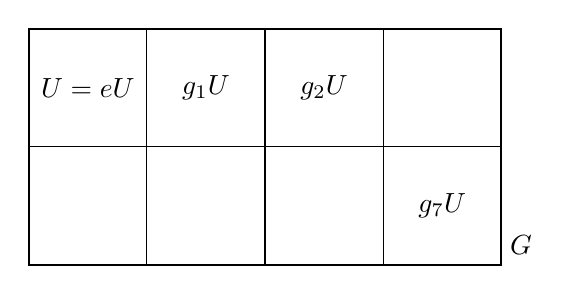
\begin{tikzpicture}
            \draw[thick] (0,0) rectangle (6, 3);
            \draw (0,1.5) -- (6,1.5) (1.5,0) -- (1.5,3) (3,0) -- (3,3) (4.5, 0) -- (4.5, 3);
            \node at (6.25, 0.25) {$G$};  
            \node at (0.75, 2.25) {$U = eU$};
            \node at (2.25, 2.25) {$g_1U$};
            \node at (3.75, 2.25) {$g_2U$};
            \node at (5.25, 0.75) {$g_7U$};
        \end{tikzpicture}
        \caption{Nebenklassenzerlegung einer endlichen Gruppe}
    \end{figure}
\end{remark}

\begin{remark}
    Es gilt auch für Gruppen mit unendlicher Trägermenge, dass es gleich viele Linksnebenklassen wie Rechtsnebenklassen gibt. Es kann dafür die Funktion $\varphi: gU \mapsto Ug^{-1}$ definiert werden und gezeigt werden, dass diese wohldefiniert und bijektiv ist.
\end{remark}

\begin{theorem}[Lagrange]\index{Satz!von Lagrange}
    Sei $G$ eine endliche Gruppe, $U \le G$ eine Untergruppe und $g \in G$. Dann gilt
    \begin{itemize}[topsep=0cm, label={--}]
        \item $\vert U \vert$ teilt $\vert G \vert$ und
        \item $\ord(g)$ teilt $\vert G \vert $.
    \end{itemize}
\end{theorem}
\begin{proof}
    Die erste Behauptung folgt aus \cref{rem:nebenklassenzerlegung_endlich}, für die zweite wählen wir $U := \langle g \rangle$.
\end{proof}

\begin{example}
    Betrachten wir $(\mathbb{Z}_6, +, 0, -)$ mit Ordnung 6. Es sind dann $\ord(0) = 1, \ord(1) = \ord(5) = 6, \ord(2) = \ord(4) = 3, \ord(3) = 2$, welche alle Teiler von 6 sind.

    Sei $G$ eine Gruppe mit $\vert G \vert = p \in \mathbb{P}$. Für $g \in G\setminus\{e\}$ gilt nun $\ord(g) = p \Rightarrow \langle g \rangle = G$, womit $G$ zyklisch ist. Gruppen mit Primzahlordnung sind also zyklisch.
\end{example}

\begin{definition}
    Sei $G$ eine Gruppe und $U \le G$ eine Untergruppe. Der \emph{Index von $U$ in $G$}\index{Index} ist definiert als $[G:U] := \vert \{gU \mid g \in G\}\vert = \vert \{Ug \mid g \in G\}\vert$. 
\end{definition}

\begin{remark}
    Ist $G$ endlich, dann haben wir in \cref{rem:nebenklassenzerlegung_endlich} $[G:U] = \frac{\vert G \vert}{\vert U \vert}$ gezeigt.
\end{remark}

\begin{theorem}[Indexsatz]\index{Indexsatz}
    Sei $G$ eine Gruppe und seien $U \le V \le G$ Untergruppen, dann ist $$[G:V] = [G:U] \cdot [U:V].$$ 
\end{theorem}
\begin{proof}
    Wurde in der Übung bewiesen.
\end{proof}

Im Allgemeinen ist die durch Links-/Rechtsnebengruppen induzierte Äquivalenzrelation keine Kongruenzrelation. Der folgende \cref{theorem:normalteiler_equiv} liefert Bedingungen, wann dies erfüllt ist.

\begin{definition}
    Sei $G$ eine Gruppe, dann heißt eine Teilmenge $N \subseteq G$ \emph{Normalteiler}\index{Normalteiler}, wenn eine der Bedingungen aus \cref{theorem:normalteiler_equiv} erfüllt ist. Man schreibt $N\vartriangleleft G$.
\end{definition}

\begin{theorem}\label{theorem:normalteiler_equiv}
    Sei $G$ eine Gruppe, $N \subseteq G$, dann sind äquivalent:
    \begin{enumerate}[label=(\enumArabicDual*)]
        \item\label{item:theorem:normalteiler_equiv_1} Es gibt genau eine Kongruenzrelation $\sim$ auf $G$ mit $N = [e]_\sim$, nämlich $x \sim y: \Leftrightarrow x^{-1}y \in N$.
        \item\label{item:theorem:normalteiler_equiv_1'} Es gibt eine Kongruenzrelation $\sim$ auf G mit $N = [e]_\sim$.
        \item\label{item:theorem:normalteiler_equiv_2} Es gibt eine Gruppe $H$ und einen surjektiven Homomorphismus $\varphi: G \to H$ mit $N = \varphi^{-1}(\{e_H\})$.
        \item\label{item:theorem:normalteiler_equiv_2'} Es gibt eine Gruppe $H$ und einen Homomorphismus $\varphi: G \to H$ mit $N = \varphi^{-1}(\{e_H\})$.
        \item\label{item:theorem:normalteiler_equiv_3} Es ist $N \le G$ mit $\forall x \in G: xNx^{-1} = N$.
        \item\label{item:theorem:normalteiler_equiv_3'} Es ist $N \le G$ mit $\forall x \in G: xNx^{-1} \subseteq N$.
        \item\label{item:theorem:normalteiler_equiv_4} Es ist $N \le G$ mit $\forall x \in G: xN = Nx$.
        \item\label{item:theorem:normalteiler_equiv_4'} Es ist $N \le G$ mit $\forall x \in G: xN \subseteq Nx$.
    \end{enumerate}
\end{theorem}


\begin{proof}{\ }
    \begin{itemize}[topsep=0cm, leftmargin=2.2cm]
        \item[\ref*{item:theorem:normalteiler_equiv_1} $\Rightarrow$ \ref*{item:theorem:normalteiler_equiv_1'}:] 
        Trivial.
        
        \item[\ref*{item:theorem:normalteiler_equiv_1'} $\Rightarrow$ \ref*{item:theorem:normalteiler_equiv_2}:] 
        Wählen wir $H = G/_\sim$ und sei $\varphi: G \to H, g \mapsto [g]_\sim$ die kanonische Einbettung. Es ist dann klarerweise $\varphi$ surjektiv und $\varphi^{-1}(\{e_H\}) = [e]_\sim = N$.
        
        \item[\ref*{item:theorem:normalteiler_equiv_2} $\Rightarrow$ \ref*{item:theorem:normalteiler_equiv_2'}:] 
        Trivial.
        
        \item[\ref*{item:theorem:normalteiler_equiv_2'} $\Rightarrow$ \ref*{item:theorem:normalteiler_equiv_3'}:] 
        Zeigen wir zuerst, dass $N$ eine Untergruppe ist. Seien dazu $n, n' \in N = \varphi^{-1}(\{e_H\})$. Dann ist $\varphi(n n') = \varphi(n) \varphi(n') = e_H e_H = e_H$, womit $n n' \in \varphi^{-1}(\{e_H\}) = N$ ist und damit $N \le G$.

        Zeigen wir nun noch für $x \in G, n \in N$, dass $y = xnx^{-1} \in N$ ist. Wir erhalten $$\varphi(y) = \varphi(x) \underbrace{\varphi(n)}_{= e_H} \varphi(x^{-1}) = \varphi(x)\varphi(x)^{-1} = e_H \;\Rightarrow\; y \in \varphi^{-1}(\{e_H\}) = N.$$

        \item[\ref*{item:theorem:normalteiler_equiv_3'} $\Rightarrow$ \ref*{item:theorem:normalteiler_equiv_3}:] 
        Wir wissen bereits, dass $\forall x \in G: xNx^{-1} \subseteq N$ gilt und wollen zeigen, dass für $y \in G$ die umgekehrte Inklusion gilt. Es ist $y^{-1} \in G$, womit $y^{-1}N(y^{-1})^{-1} = y^{-1}Ny \subseteq N$ ist. Wir erhalten damit nun 
        $$ N \overset{(*)}{=} y y^{-1} N y y^{-1} = y (y^{-1} N y) y^{-1} \subseteq y N y^{-1}, $$
        wobei $(*)$ einfach nachzurechnen ist.
        
        \item[\ref*{item:theorem:normalteiler_equiv_3} $\Rightarrow$ \ref*{item:theorem:normalteiler_equiv_4}:] 
        Zeigen wir für $x \in G$, dass $xN \subseteq Nx$ ist. Für ein $y \in xN$ gibt es ein $n \in N$, sodass $y = xn$. Wählen wir $n' = yx^{-1} = xnx^{-1} \in xNx^{-1} = N$, so ist $y = n'x$ und damit $y \in Nx$. Die andere Mengeninklusion zeigt man analog. 
        
        \item[\ref*{item:theorem:normalteiler_equiv_4} $\Rightarrow$ \ref*{item:theorem:normalteiler_equiv_4'}:] 
        Trivial.
        
        \item[\ref*{item:theorem:normalteiler_equiv_4'} $\Rightarrow$ \ref*{item:theorem:normalteiler_equiv_1}:]  
        Zeigen wir zuerst die Eindeutigkeit: Sei angenommen es gibt eine Kongruenzrelation $\sim$ auf $G$ mit $N = [e]_\sim$. Für $x, y\in G$ gilt dann 
        \begin{itemize}[label={--}]
            \item $x \sim y \;\Rightarrow\; x^{-1}x \sim x^{-1}y \; \Leftrightarrow\; e \sim x^{-1}y \;\Leftrightarrow\; x^{-1}y \in [e]_\sim = N$ und
            \item $x^{-1}y \in N = [e]_\sim \;\Leftrightarrow\; e \sim x^{-1}y \;\Leftrightarrow\; x = xe \sim x(x^{-1}y) = y$.
        \end{itemize}
        Es ist dann also $x \sim y \Leftrightarrow x^{-1}y \in N$. 
        
        Zeigen wir nun noch, dass dieses $\sim$ eine Kongruenzrelation auf $G$ ist. Nach \cref{lemma:euqivrel_linksnebenklassen} ist $\sim$ eine Äquivalenzrelation, bleibt also noch die Invarianz unter $G$ zu zeigen. 
        \begin{itemize}[label={--}]
            \item Zeigen wir für $x,x',y,y' \in G$ mit $x \sim y, x' \sim y'$, dass $xx'\sim yy'$. Es gilt 
            $$ xx'\sim yy' \;\Leftrightarrow\; x'^{-1}\underbrace{x^{-1}y}_{=: n \in N} y' = \underbrace{x'^{-1} n}_{\in x'^{-1}N \subseteq Nx'{-1}} y' \overset{(*)}{=} n'\underbrace{x'^{-1}y'}_{\in N} \in N, $$
            wobei wir bei $(*)$ verwenden, dass nach \ref*{item:theorem:normalteiler_equiv_4'} ein $n' \in N$ existiert, sodass $x'{-1} n = n' x'{-1}$.
            \item Zeigen wir für $x,y \in G$ mit $x \sim y$, dass $x^{-1} \sim y^{-1}$. Es gilt
            $$ x\sim y \;\Leftrightarrow\; x^{-1}x \sim x^{-1}y \;\Leftrightarrow\; e \sim x^{-1}y \;\Leftrightarrow\; ey^{-1} \sim x^{-1} y y^{-1} \;\Leftrightarrow\; y^{-1} \sim x^{-1}.$$ 
            \item Klarerweise ist $e \sim e$, also ist $\sim$ invariant unter der 0-stelligen Operation $e$.
        \end{itemize}
    \end{itemize}
\end{proof}

\begin{remark}
    \cref{theorem:normalteiler_equiv} beschreibt einige Eigenschaften von Normalteilern.
    \begin{itemize}[label={--}]
        \item \ref*{item:theorem:normalteiler_equiv_1}, \ref*{item:theorem:normalteiler_equiv_1'} liefern den bijektiven Zusammenhang von Normalteilern und Kongruenzrelation. Betrachtet man die Verbände von Normalteilern bzw. Kongruenzrelationen, so stellt diese Bijektion einen Verbandsisomorphismus dar.
        \item \ref*{item:theorem:normalteiler_equiv_2}, \ref*{item:theorem:normalteiler_equiv_2'} beschreiben die Darstellung des Normalteilers über den Kern eines Homomorphismus $\varphi: G \to H$. Es ist $\ker \varphi = \{g \in G \mid \varphi(g) = e_H\} = \varphi^{-1}(\{e_H\}) = N$.
        \item \ref*{item:theorem:normalteiler_equiv_3}, \ref*{item:theorem:normalteiler_equiv_3'} liefern direkt, dass Normalteiler unter Abbildungen $\pi_x: G \to G, g \mapsto xgx^{-1}$ abgeschlossen sind. So eine Abbildung nennt man \emph{inneren Automorphismus}.
        \item \ref*{item:theorem:normalteiler_equiv_4}, \ref*{item:theorem:normalteiler_equiv_4'} besagen, dass die Links- und Rechtsnebenklassen genau dann gleich sind, wenn die Untergruppe ein Normalteiler ist.
    \end{itemize}

    Inbesondere sind alle Äquivalenzklassen einer Kongruenzrelation gleich groß, da sie lediglich ``Verschiebungen'' der Äquivalenzklasse des neutralen Elements sind.
\end{remark}

\begin{corollary} \label{corollary:abelsch-normalteiler-untergruppe}
    In einer abelschen Gruppe $G$ ist $N \subseteq G$ genau dann ein Normalteiler, wenn $N$ eine Untergruppe von $G$ ist.
\end{corollary}
\begin{proof}
    In einer abelschen Gruppe ist immer $xN = Nx$. \cref{theorem:normalteiler_equiv} \ref*{item:theorem:normalteiler_equiv_4} liefert dann damit die Behauptung.
\end{proof}

\notedate{19.04.2023}

\begin{remark} \label{remark:gruppe-injektiv-kern-trivial}
    Seien $G, H$ Gruppen, $h : G \to H$ ein Homomorphismus. Es sei erinnert, dass $h$ injektiv ist, wenn
    $$ \{ (x,y) \mid h(x) = h(y) \} = \{ (x,x) \mid x \in G \}. $$
    Diese Menge definiert eine Kongruenzrelation $\sim$ auf $G$. Also ist $h$ genau dann injektiv, wenn $[e]_\sim = \{e\}$, also gerade $\ker h = \{ e \}$. Man vergleiche diese Eigenschaft mit der Injektivität von Vektorraum-Homomorphismen aus der Linearen Algebra.
\end{remark}

\begin{remark}
    Es sei an \cref{def:einfache-algebra} einer einfachen Algebra erinnert. Wir bemerken, dass eine Gruppe genau dann einfach ist, wenn sie nur ihre Trägermenge und $\{e\}$ als Normalteiler hat.
\end{remark}

\begin{definition}
    Sei $G$ eine Gruppe, $N \vartriangleleft G$ ein Normalteiler und $\sim$ die entsprechende Kongruenzrelation. Wir definieren die \emph{Faktorgruppe} \index{Gruppe!Faktor-}
    $$ G /_\sim = \{ aN \mid a \in G \}. $$
    Dabei ist
    $$ aN \cdot bN := (a \cdot b)N. $$
    Man überzeugt sich leicht davon, dass dies gerade dann wohldefiniert ist wenn eben $N$ ein Normalteiler ist.
\end{definition}

\begin{example}
    Betrachte die Gruppe $(\mathbb{Z}, +, 0, -)$, so ist für jedes $m \in \mathbb{N}$ die Menge $m \mathbb{Z}$ eine Untergruppe, und da sie kommutativ ist nach \cref{corollary:abelsch-normalteiler-untergruppe} auch ein Normalteiler.

    Sei $\sim$ die entsprechende Kongruenzrelation und betrachten wir $(\mathbb{Z}, +, 0, -)/_\sim$, so enthält diese Faktorgruppe
    $$ 0 + m\mathbb{Z}, \quad 1 + m\mathbb{Z}, \quad \hdots, \quad (m-1) + m\mathbb{Z}. $$

    In dieser Gruppe rechnet man
    $$ (i + m\mathbb{Z}) + (j + m\mathbb{Z}) = (i+j) + m\mathbb{Z}, $$
    wobei man auch $(i + j \pmod{m})$ für einen ``schöneren'' Repräsentanten betrachten kann.

    Im Falle $n = 4$ ist beispielsweise
    $$ (1 + 4\mathbb{Z}) + (3 + 4\mathbb{Z}) = 4 + 4\mathbb{Z} = 0 + 4\mathbb{Z}. $$
\end{example}

\begin{example}
    Betrachte die Gruppe $(\Gl_2(\mathbb{R}), \cdot, E_2, {}^{-1})$ und
    $$ N := \{ A \in \Gl_2(\mathbb{R}) \mid \det A = 1 \}. $$
    Für ein beliebiges $A \in \Gl_2(\mathbb{R})$ gilt $ A N A^{-1} \subseteq N, $ da mit $C \in N$
    $$ \det(A C A^{-1}) = \det A \det N \det A^{-1} = \det C = 1. $$
    Also ist $N$ ein Normalteiler. Sei $\sim$ die entsprechende Äquivalenzrelation, wir wollen die Struktur von $\Gl_2(\mathbb{R})/_\sim$ analysieren. Es gilt
    $$ A \sim B \Leftrightarrow A \cdot B^{-1} \in N \Leftrightarrow \det(A \cdot B^{-1}) = 1 \Leftrightarrow \det A = \det B, $$
    die Äquivalenzklassen hängen also nur von der Determinante und ansonsten nicht von der unterliegenden Matrixstruktur ab. Also ist $\Gl_2(\mathbb{R})/_\sim \cong (\mathbb{R} \setminus \{0\}, \cdot, 1, {}^{-1})$.
\end{example}

\begin{remark}
    Sei $G$ eine Gruppe, $\sim$ eine Kongruenzrelation. Wir fragen uns, wann $G/_\sim$ kommutativ ist. Dazu bemerken wir
    $$ G/_\sim \textrm{ kommutativ} \quad \Leftrightarrow \quad \forall a, b \in G: (ab)N = (aN) (bN) = (bN) (aN) = (ba)N. $$
    Letzteres können wir umschreiben als $a^{-1} b^{-1} a b N = N$, was genau dann der Fall ist, wenn für beliebiges $a, b$ gilt
    $$ [a, b] := a^{-1} b^{-1} a b \in N. $$
    Wir nennen $[a, b]$ den \emph{Kommutator} \index{Kommutator} von $(a, b)$.
\end{remark}

\begin{definition}
    Definiere
    $$ G' := \langle \{ [a, b] \mid a, b \in G \} \rangle \leq G. $$
    Wir nennen $G'$ die \emph{Ableitung} oder auch die \emph{Kommutatorgruppe} von $G$. \index{Gruppe!Ableitung}\index{Gruppe!Kommutatorgruppe}
\end{definition}
    
\begin{proposition}
    Sei $G$ eine Gruppe. Ist $G$ abelsch, so ist $G' = \{ e \}$.
\end{proposition}

\begin{proof}
    Ist $G$ abelsch so ist
    $$ G' = \langle \{ a^{-1} b^{-1} a b \mid a, b \in G \} \rangle = \langle \{ a^{-1} b^{-1} b a \mid a, b \in G \} \rangle = \langle \{e\} \rangle = \{e\}. $$
\end{proof}

\begin{theorem}
    Sei $G$ eine Gruppe. Dann gilt:
    \begin{enumerate}
        \item $G' \vartriangleleft G$
        \item $G/_{G'}$ ist abelsch.
        \item $\forall N \vartriangleleft G: ( G/_N \textrm{ abelsch} \Leftrightarrow N \supseteq G')$
    \end{enumerate}
\end{theorem}

\begin{proof}
    (2) ist ein Spezialfall von (3).

    Um (3) einzusehen sei $N \vartriangleleft G$, so folgt mit obiger Bemerkung sofort
    \begin{align*}
        G/_N \textrm{ abelsch} &\Leftrightarrow \forall a, b: (aN)(bN) = (bN)(aN) \Leftrightarrow \\ &\Leftrightarrow \forall a, b a^{-1}b^{-1} a b \in N \Leftrightarrow \forall a, b: [a, b] \in N \Leftrightarrow N \subseteq G'.
    \end{align*}

    Zeigen wir nun (1). Sei $h : G \to G$ ein beliebiger Endomorphismus, dann gilt für alle $a, b \in G$, dass $h([a,b]) = [h(a), h(b)]$, also $h(G') \subseteq G'$. Für beliebiges $x \in G$ definieren wir
    $$ h_x : G \to G, g \mapsto xgx^{-1}, $$
    so ist $h_x$ ein Automorphismus\footnote{$h_x$ ist wie früher schon bemerkt ein \emph{innerer Automorphismus}.}. Also ist
    $$ x G' x^{-1} = h_x(G') \subseteq G', $$
    womit $G' \vartriangleleft G$ folgt.
\end{proof}

\begin{definition}
    Sei $G$ eine Gruppe, $U_1, U_2 \subseteq G, x \in G$, so definieren wir das \emph{Komplexprodukt}
    $$ U_1 \cdot U_2 = \{ u_1 \cdot u_2 \mid u_1 \in U_1, u_2 \in U_2 \}. $$
\end{definition}

\begin{definition} \label{def:direktes-inneres-produkt}
    Sei $G$ eine Gruppe, $U_1, \hdots, U_n \leq G$. Wir nennen $G$ ein \emph{inneres direktes Produkt} von $(U_1, \hdots, U_n)$, wenn die Abbildung
    $$ \varphi : U_1 \times \hdots \times U_n \to G, (u_1, \hdots u_n) \mapsto u_1 \cdot \hdots \cdot u_n $$
    ein Isomorphismus ist. In diesem Fall schreiben wir $G = U_1 \odot \hdots \odot U_n$.
\end{definition}

\begin{remark} \label{remark:inneres-direktes-produkt-notwendig}
    Wir sammeln nun notwendige Bedingungen dafür, dass $G$ ein inneres direktes Produkt ist.
    
    Für $i \in \{ 1,\hdots,n \}$ definiere $V_i := U_1 \cdot \hdots \cdot U_{i-1} \cdot U_{i+1} \cdot \hdots \cdot U_n$, so muss gelten
    $$ U_i \cap V_i = \{ e \}. $$
    Sonst gäbe es $(u_j)_{j=1}^n \in (U_j)_{j=1}^n, u_i \neq e$ mit
    $$ \varphi(e, \hdots, e, \overbrace{u_i}^{\textrm{$i$-te Stelle}}, e, \hdots, e) = u_i \overset{!}{=} u_1 \cdot \hdots \cdot u_{i-1} \cdot u_{i+1} \cdot \hdots \cdot u_n = \varphi(u_1, \hdots, u_{i-1}, e, u_{i+1}, \hdots, u_n), $$
    womit $\varphi$ nicht injektiv wäre.

    Weiters muss $U_i \vartriangleleft G$ sein. Um dies einzusehen, betrachte die Abbildung
    $$ \psi_i : U_1 \times ... \times U_n \to U_1 \times ... \times U_{i-1} \times U_{i+1} \times ... \times U_n, (u_i)_{i=1}^n \mapsto (u_i, \hdots, u_{i-1}, u_{i+1}, \hdots, u_n). $$
    Diese ist ein Homomorphismus, womit
    $$ \ker \psi_i = \{e\} \times ... \times \{e\} \times U_i \times \{e\} \times ... \times \{e\} \vartriangleleft U_1 \times ... \times U_n. $$
    Damit ist $U_i = \varphi(\ker \psi_i) \vartriangleleft G$.

    Zuletzt gilt in einem direkten inneren Produkt für $i \neq j, x \in U_i, y \in U_j$, dass $xy = yx$. Um dies einzusehen sei \obda $i < j$, so gilt
    \begin{align*}        
        xy &= \varphi(e, \hdots, e, \overbrace{x}^{\textrm{$i$-te Stelle}}, e, \hdots, e) \cdot \varphi(e, \hdots, e, \overbrace{y}^{\textrm{$j$-te Stelle}}, e, \hdots, e) =  \\ &= \varphi(e, \hdots, e, \overbrace{x}^{\textrm{$i$-te Stelle}}, e, \hdots, e, \overbrace{y}^{\textrm{$j$-te Stelle}}, e, \hdots, e) = \\ &= \varphi(e, \hdots, e, \overbrace{y}^{\textrm{$i$-te Stelle}}, e, \hdots, e) \cdot \varphi(e, \hdots, e, \overbrace{x}^{\textrm{$j$-te Stelle}}, e, \hdots, e) = yx.
    \end{align*}
\end{remark}

\begin{lemma} \label{lemma:gruppe-normalteiler-kommutativ}
    Sei $G$ eine Gruppe, $U, V \vartriangleleft G$, $U \cap V = \{ e \}$, dann gilt für alle $u \in U$ und $v \in V$, dass $uv = vu$.
\end{lemma}

\begin{proof}
    Es gilt
    $$ uv = vu \Leftrightarrow u^{-1} v^{-1} u v = e. $$
    Nun ist $u^{-1} v^{-1} u \in V$, damit $u^{-1} v^{-1} u v \in V$. Andererseits gilt $v^{-1} u v \in U$, damit $u^{-1} v^{-1} u v \in U$. Also folgt $u^{-1} v^{-1} u v = e$ und damit $uv=vu$.
\end{proof}

\begin{proposition} \label{prop:kriterien-direktes-inneres-produkt}
    Sei $G$ eine Gruppe und $U_1, \hdots, U_n \leq G$. Gelte $G = U_1 \cdot \hdots \cdot U_n$, beziehungsweise äquivalent die Surjektivität von $\varphi$ wie in \cref{def:direktes-inneres-produkt}. Gelte weiters für $i \in \{ 1, \hdots, n \} $, dass $U_i \vartriangleleft G$ und $U_i \cap V_i = \{ e \} $, wobei $V_i$ wie in \cref{remark:inneres-direktes-produkt-notwendig} definiert ist. Dann ist $G = U_1 \odot \hdots \odot U_n $.
\end{proposition}

\begin{proof}
    Definiere $\varphi$ wie in \cref{def:direktes-inneres-produkt}, so ist $\varphi$ nach Voraussetzung surjektiv.

    Zeigen wir, dass $\varphi$ ein Homomorphismus ist. Mit \cref{lemma:gruppe-normalteiler-kommutativ} gilt
    \begin{align*}        
        \varphi((u_1, \hdots, u_n) \cdot (v_1, \hdots, v_n)) &= \varphi(u_1 v_1, \hdots, u_n v_n) = u_1 v_1 \hdots u_n v_n = \\ &= u_1 \hdots u_n v_1 \hdots v_n = \varphi(u_1, \hdots, u_n) \varphi(v_1, \hdots, v_n).
    \end{align*}

    Bleibt die Injektivität zu zeigen. Dazu reicht es nach \cref{remark:gruppe-injektiv-kern-trivial} zu zeigen, dass der Kern trivial ist. Sei also $\varphi(u_1, \hdots, u_n) = e$, so ist $(u_1, \hdots, u_n) = (e, \hdots, e)$ zu zeigen. Sei dazu indirekt angenommen es wäre nicht der Fall und sei $i$ minimal mit $u_i \neq e$, also
    $$ e = \varphi(u_1, \hdots, u_n) = e \hdots e u_i \hdots u_n = u_i \hdots u_n, $$
    womit $u_i^{-1} = u_{i+1} ... u_n \in V_i$ folgt. Da jedoch auch $u_i^{-1} \in U_i$ und $U_i \cap V_i = \{ e \}$ folgt damit $u_i = e$, im Widerspruch.

    Insgesamt ist $\varphi$ also ein Isomorphismus, was zu zeigen war.
\end{proof}

\begin{remark}
    Sei $(U_i)_{i \in I}$ eine Familie von Untergruppen einer Gruppe $G$, wobei $(I, <)$ totalgeordnet ist. Wir definieren das \emph{schwache Produkt} \index{schwaches Produkt}
    $$ \prod_{i \in I}^w U_i := \{ f : I \to \bigcup_{i \in I} U_i \mid \forall i \in I: f(i) \in U_i \land f(i) = e \textrm{ für fast alle } i \in I \}. $$
    Definiere weiters
    $$ \varphi : \prod_{i \in I}^w U_i \to G, f \mapsto f(i_1) \cdot \hdots \cdot f(i_k), $$
    wobei $i_1 < \hdots < i_k $ genau jene Indizes sind, für die $f(i_j) \neq e$ ist.

    Falls $\varphi$ ein Isomorphismus ist, so nennen wir $G$ \emph{inneres direktes Produkt} von $(U_i)_{i \in I}$.

    Ohne Beweis sei angemerkt dass \cref{prop:kriterien-direktes-inneres-produkt} entsprechend auch für solche inneren direkten Produkte gilt.
\end{remark}